\def \coursename  {CM3070 CS Final Project}
\def \assigntment {Final Project Report}
\author {Hayato Ishida}

\documentclass[11pt, natbib=false]{article}

\usepackage{url}
\usepackage{hyperref}
\usepackage{fancyhdr}
\usepackage{multicol}
\usepackage{listings}


\setlength{\columnsep}{1cm}
\usepackage[backend=bibtex,
            sorting=none,
            citestyle=numeric,
            style=ACM-Reference-Format]{biblatex}
\addbibresource{refrence.bib}
\usepackage{geometry}
\geometry{margin=2.5cm}

\usepackage{graphicx}
\usepackage{subcaption}
\usepackage{hyperref}

\setlength\parindent{2em}
\setlength\parskip{0em}
\renewcommand{\baselinestretch}{1.5}
\linespread{1.3}

% \pagestyle{fancyplain}
% \chead{\assigntment}
\date{\today}
\title{%
  Developing the ML Model With Genetic Algorithm \\
  \large BSc Computer Science Final Project
}


\begin{document}

\maketitle
\href{https://github.com/hayacon/cs_final_project}{Link to GitHub repository of this project}

The dataset of this project may contain comments with offensive or abusive language.
% \begin{multicols}{2}
\section{Introduction}
These days, many human-to-human interactions are taking place on online platforms, mainly on social media.
Many comments are being exchanged on a wide range of topics within social media, but that does not mean that it is all necessarily appropriate ~\cite{hada2021ruddit}.
Some of the contents may include offensive or hateful language, and exposure to those contents can affect users’ mental health, and well-being ~\cite{hada2021ruddit}.

In March of 2020, COVID-19 pandemic was declared by WHO ~\cite{whoCovid}.
Since then, many countries have placed various major restrictions to fight this disease, including social distancing and lockdowns. Social media plays a vital role in connecting people during that time. Although it brought lots of benefits to our society, there is also a dark side ~\cite{liu2021covid}.
A study ~\cite{babvey2021using} shows an increase in abusive content or comments on Twitter and Reddit in several countries, specifically countries with strong restrictions.
For instance, in Japan, a young TV star, Hana Kimura, committed suicide after reading hurtful and offensive comments online ~\cite{HanaK}.
Following this incident, there was a lot of attention paid to cyber bullying, and comments with abusive language. The Government of Japan had even considered enforcement of punishments towards those who use offensive language on social media platforms. ~\cite{JpGov}.


A system for detecting offensive, abusive and hateful content is attracting more interest from social media platforms and regulators ~\cite{vidgen2019challenges}.
Reason being is that, there is a growing concern about the effects on the mental health of the younger generation that consume this content ~\cite{babvey2021using}.
However, due to the ambiguous and diverse definitions of offensive content, it is a challenging topic for the research field of NLP and machine learning ~\cite{vidgen2019challenges}.

This project attempts to develop a machine learning model that overcome several challenges, classifying diverse offensive content and understanding short text.
This model should identify the degree of offensiveness and convert it into a numerical value instead of labeling it under a specific class.
Also, it can be used as a solution to overcome the ambiguity and diverseness of offensive content.
It will also use genetic algorithms to automate the optimization process of neural network architecture ~\cite{andersen2021evolving}. 
This genetic algorithm is a searching algorithm inspired by the theory of evolution developed by Charles Darwin in 1859.
With this algorithm, the neural network can possibly be developed automatically.

This project is based on the final project template of Machine Learning and Neural Network: deep learning on a public dataset.
In addition, the project is partially inspired by the Artificial Intelligence project template: automated design using evolutionary computation.
Also, includes knowledge and programming techniaues of Natural Language Processing. 

\section{Literatures Review}
Since this is a well-established topic of research in Machine Learning and Natural Language Processing, there were already several studies are related to offensive language detection. 

Malmasi Shervin and Zampieri Marcos ~\cite{malmasi2017detecting} demonstrate a text classification model to classify hate speech in social media. This study developed a supervised classification model using a publicly published dataset of tweets from Twitter.
The study used surface n-gram and word skip grams features, which have proven to work well with this task. The study uses support vector machines with LIBLINEAR package for a classifier model because of their high performance with similar word classification.
The package, however, the study also demonstrates some problems with hate speech classification. First of all, each tweet of the dataset was labeled by individuals into three different classes: Hate, offensive, and ok.
There is some ambiguity of definitions between ‘hate’ and ‘offensive.’ In the usual sense, different individuals would get different impressions from the same content.
For example, with the same violent tweet, some might think it is ‘offensive,’ but others might think it is instead ‘hate.’
The result of this study exactly shows the ambiguity of those class definitions. The classification model successfully distinguishes the ‘ok’ tweet from the other two. However, the model performance was not good enough to distinguish between ‘hate’ and ‘offensive’; also, some ‘hate’ or ‘offensive’ tweets are classified as ‘ok.’
This result demonstrates that there is an overlap of definition between those three classes because of ambiguity of language.
The study shows that this is not practical to use specific classes to detect any hate or offensive content on social media platforms.
It is necessary to overcome that ambiguity of language to build a practical and effective text classification model. 

The study by Rishav Hada et al. ~\cite{hada2021ruddit} also points out those ambiguous definitions of different types of offensive languages.
This study is similar to Malmasi Shervin and Zampieri Marcos ~\cite{malmasi2017detecting} but approaches the problem differently.
Classifying offensive language is quite complicated because there are many possible classes such as racist, sexist, hate speech, offensive, hateful, etc. In the real world, those classes can be ambiguous and overlap.
In addition to those ambiguities, swear words are another problem that offensive text classification must consider.
It is easy to classify them as offensive, but text with swear words does not necessarily mean offensive.
For instance, ‘Hell yes, and ‘sure as hell love it’ are not offensive.
Those comments use swear words to express their positive emotion, however, these words surely have inappropriate uses.
This study overcomes the ambiguity of offensive words by giving each data the best-worst scaling between -1 and 1, where -1 is maximally supportive, and 1 is maximally offensive.
This approach allows classification tasks to be less ambiguous.
Although each person will take an offensive text differently, it will not cause different classes to overlap.
The study considers three different computational models: Bidirectional LSTM ~\cite{pennington2014glove}, BERT ~\cite{devlin2018bert}, and HateBERT ~\cite{caselli2020hatebert}.
As a result, HateBERT performs the best, and considering its publication date, it is a good result. 

The previous two studies give a clear insight into distinguishing between different types of offensive languages on social media or the internet platforms.
The following study shows the negative effects of offensive words on young people.

The paper by Shi Xiaoqin, Yu Chao, and Wu Dongmei ~\cite{shi2021influence} study how those violent languages on the Internet affect young students' mental health.
Most young students are users of the Internet, and it is hard to find a young student who does not have a social media account.
The study focuses on young students because they are most vulnerable to consuming hateful speech on the Internet.
Young people are in the middle of physical and mental development, and the study focuses on the negative effects of such speech during that developmental stage.
The study shows that there are many different negative effects on young students’ mental health, and an attempt of psychological intervention to improve their mental health did not bring significant positive results.
All of those negative psychological effects lead to various problems for young students.
It can cause problems in daily life activities such as sleeping, eating, interpersonal relationships, and other mental health-related problems.
Those problems can lead to other problems for young students, as well. To improve those psychological problems, the improvement of online platforms is necessary.
Unfortunately, some online platforms ignore those language violences and gain some attention to maintain or increase traffic and for another benefit.
This leads to more violence. Adults are likely to have the capability to avoid those contents or deal with those contents.
However, young people are not capable of dealing with those content. Therefore, some sort of protection is necessary for them.
Although the data sample of this study is small, it still shows the significance of those adverse effects caused by language violence on the Internet.
An efficient violent language detecting system is the possible solution for this issue. 

The study by Rishav Hada et al. ~\cite{hada2021ruddit} proposed some efficient text classification methods to detect offensive language.
The study by Andersen Hayden et al. ~\cite{andersen2021evolving} shows the possibility of using a genetic algorithm to construct an efficient text classification model automatically.
Genetic algorithm is a bio-inspired searching algorithm that can bring solutions beyond our imagination ~\cite{lehman2020surprising}.
One of the main issues in developing text classification is the requirement of knowledge.
Convolutional Neural Network is known for its high performance in text classification tasks. To develop a good text classification model with a Convolutional Neural Network, deep knowledge of natural language processing and a combination of machine learning, deep learning and neural networks are necessary.
Also, constructing this type of text classification model is not easy to do in general. Considering those challenges, this study attempt to automate the construction process by genetic algorithm.
Although it is still an initial stage of this area of research, this study shows various possibilities of applying genetic algorithms to text classification tasks.
The study shows two similar but different approaches. In genetic algorithm representation of genetic data of each model is very important, and it demonstrates two different ways: vector and tree-like graphs.
The vector representation is relatively simple and easier to work with.
On the other hand, the downside of this study is computational cost.
It requires quite a lot of computation power to run a genetic algorithm.
However, it can be controlled flexibly by adjusting population size and number of generations.
As a result, the study developed well perform text classification model.
The result of the study provides evidence that the genetic algorithm can be used for machine learning model development, and it is pretty compelling. 

A text on social media platforms or any other online platform can be pretty short. For instance, content on Twitter is relatively short. The platform has a word limit of 280 characters [15].
Classifying short text is not an easy task.
The study by Wang Haitao ~\cite{wang2021short} presents a method to tackle this difficult task.
First of all, in-text classification task, the short text is harder to deal with for some reason. One of reason is that short text lack a necessary information for text classification.
The study uses Convolutional Neural Network because of its promised performance in a text classification task. It goes through three steps to perform a short text classification.
First, it uses Jaro–Winkler similarity to detect any spelling error on text. Spell miss can lead to entirely different output in the short text.
Secondly, it finds related words to extend the semantics of short text. Finally, conceptualize short text and then extract short text features.
As a result, the study successfully improved the performance of short text classification.
Combining this technique with a traditional text classification method in a real-world application can be pretty challenging.
However, at the same time, it is a necessary technique to apply text classification to various content on online platforms. 

Those studies consider various methods to construct well perform text classification model.
Therefore, the results of those studies are a beneficial source to consider the methodology to this project of offensive language rating. 



\section{Design}
\subsection{Overview}
The main objective of this project is to develop an offensive language detection model using Machine Learning and Neural Network knowledge.
The project also involves some knowledge from Natural Language Processing and Artificial Intelligence. The model aims to detect various offensive languages on online platforms, including social media platforms and other platforms that allow users to leave a comment.
The project only considers one language, which is English.
Reasons for this will be explained in a later section.
This area of research is one of the main focuses in the Natural Language Processing research community, mainly because of increasing online platforms.
Offensive language detection is the necessary technology to keep online platforms healthy in many ways ~\cite{vidgen2019challenges}. A conventional text detecting model classifies a text into a specific class.
For instance, particularly to this project’s topic, classes can be ‘hate,’ ‘violence,’ ‘offensive.’ ‘ok,’ etc. The language is often very ambiguous, and it is always a challenge that natural language processing face.
Of course, this ambiguity applies to offensive language, as well. Categorization is a crucial part of modeling the Machine Learning model.
Categorization is complex in offensive language because of its variety ~\cite{vidgen2019challenges}.
There are many possible ways to categorize them. The general approach would be to categorize them into simple classes such as ‘hate,’ ‘offensive,’ ‘ok,’ etc. However, different researchers use a different level of abstraction and can be pretty unclear ~\cite{vidgen2019challenges}.
There is research ~\cite{malmasi2017detecting} that shows results that demonstrate how abstracted class categorization is complex for the Machine Learning model, particularly for this area of research.
To overcome this challenge, a study by a group of researchers from the Alan Turing Institute ~\cite{vidgen2019challenges} proposed a different way of categorizing offensive language.
Also, the study by Rishav Hada ~\cite{hada2021ruddit} proposes rating each text with a degree of offensiveness which is a pretty different approach compared to the conventional Machine Learning model.
This project uses a second approach to construct a Machine Learning model.
When constructing a Machine Learning model, tuning parameters can be quite challenging.
Also, it will require much time and human resources, in this case, myself.
This project will use a genetic algorithm to automatically tune parameters for building Machine Learning models and construct Neural Networks.
A genetic algorithm can take a long time to run, but it can run without the presence of a human.
Also, this will be interesting to see what level of creativity can genetic algorithm provide to construct a deep Machine Learning model.
There is one more thing that the project needs to consider, which is short text classification.
Since short text lacks the necessary contextual information to train the Machine Learning model ~\cite{wang2021short}.
Online platforms and social network platforms are full of short text.
This part might become necessary to this project, but it is not the main focus. 

\subsection{Templeate of this project}
The main template of this project is Deep Learning on a public dataset from CM3015 Machine Learning and Neural Networks. Also, this project overlaps with another template: Automated design using evolutionary computation from CM3020 Artificial Intelligence. In addition to these templates, some knowledge from CM3070 Natural Language Processing will contribute to this project. 

\subsection{Domain and users}
The primary users for this project are young adult internet users and online platform providers such as social network platforms.
Most young adults are users of various online platforms, and not all platforms have proper regulations and technologies against offensive languages.
The various negative effects of offensive language from the online platform are concerning ~\cite{babvey2021using}~\cite{shi2021influence}.
Also, it became essential for online service providers to have a robust system to detect offensive languages to provide safe platforms ~\cite{vidgen2019challenges}.
This project can also contribute to various psychological research related to negative psychological effects on mental health, such as the study about young students’ mental health ~\cite{shi2021influence}.

Inappropriate language detecting application is the primary domain for this project.
Protecting people’s mental health from offensive language is also a part of the domain.
This technology area is still considered a challenging area of research, and not all online platform providers can adopt those into their service.
Also, big technology companies have already placed systems to reduce the amount of offensive language within service, but there is still room for improvement.
Nevertheless, this area of research can contribute to protecting people’s mental health against unhealthy online behaviors. 

Today, the Internet is available in most places in the World and even in space.
Therefore, hundreds of different languages are used on various online platforms.
This project focuses on English because it is one of the most common languages in the World.
However, it is possible to apply this project to other languages in further works to reach a broader range of users.
Offensives language detecting systems related works perform well.
However, it sometimes detects regular comments as offensive or offensive language gets around the system.
Also, there is a challenge with an unclear categorization of offensive language and overall ambiguity of offensive language.
Overcoming those challenges can provide a better detecting system.
Furthermore, it is automating tuning process can implementation process more accessible for those online platform providers and make this project adaptable to different topics of text classification. 

\subsection{Overall Structure}
This project will follow the basic steps of deep learning model development.
The first steps will be data installation and pre-processing.
This process involves installing all necessary datasets into a machine’s local environment.
Then pre-process these datasets as necessary, including formatting, data cleaning, and split into train, test, validation datasets.
In the second step, the project will carry out some data analysis on the dataset to better understand the dataset, which includes some fundamental Natural Language analysis.
The actual deep learning model construction will take place next.
The base model will be from the research ~\cite{hada2021ruddit}, which shows the most effective and relates to this project the most.
However, the project will consider different choices from other related works.
As part of model construction, a genetic algorithm will search for the best-performing parameter combination. 

In this project, there are various technologies involved.
The most important technologies are the deep learning model, which consists of various knowledge, including Machine Learning and Neural networks.
Also, knowledge of Natural Language is vital for this project to succeed.
In addition, genetic algorithms play an essential role in automating some parts of the project and provide some creativity.

Another important aspect of this project is evaluation.
The result of model performance will be analyzed with Pearson correlation, MSE, and error analysis as the study by Rishav Hada ~\cite{hada2021ruddit} analyzes their data.
To evaluate this project, the result will be compared with other related works.
Since rating offensive language with numerical values is somewhat subjective, testing will require a third party to see the result.
However, this type of test can be carried out with some users. 

\subsection{Evaluation}
The aim of this project is to predict an offensive score of each comments.
Since output of prediction will be numerical value, simple evaluation method for general machine learning problem cannot be apply.
In training process, a model is constantly evaluate with MSE (mean squared error) loss function.

After training is complete, a model will evaluate with MSE.
Then, I will carry out evaluation with confusion matrix adjusted to this specific project, and also evaluation by calculating accuracy of the model’s prediction.
In addition to those evaluations, a model will also compare with baseline model, and models from a Ruddit research paper ~\cite{hada2021ruddit}.


\subsection{Project Plan}
Project planning is a crucial criterion for a successful project.
Detail plan for this project is gathered on one Gantt chart below ((a) Gantt Chart on Figures section).
The plan is set weekly, and the week count is the same as the UoL module scheduling system.
It starts from Week 9, the following week of peer graded assignment submission for project design.
There are some extra weeks of work plan in important parts of this project.
Last 5 weeks of implementation are dedicate towards evaluation, testing and implementation of a model.
Testing and evaluation are critical part of the project, and project can be improved based on result of those.
For a write up task, additional draft is included to make sure its quality is high at the final submission.
Also, for that purpose, the last 2 weeks of the project is dedicate for write up only.
Also, those extra weeks are for cases where thighs did not go as planned.
Putting some insurance in planning ensures that the project will be completed on time. 


\section{Implemementation}
Source code is availble on this project's \href{https://github.com/hayacon/cs_final_project}{GitHub repository}
\subsection{Overviwe}
The main objective of this project is to develop an offensive language detection deep learning model with the genetic algorithm.
The model aims to classify offensive languages on the scale of -1 (not offensive) and 1 (very offensive).
In addition, the genetic algorithm will be used to automatically improve the model, which is the main objective of the implementation stage of this project.
The first implementation cycle is focused on developing a baseline model.
Then, in further cycles, it focused on developing the genetic algorithm and running it to develop a well-performing machine learning model.

The project is developed with Python and various tools.
For machine learning and deep learning, I used TensorFlow and Keras.
In addition to those two, the transformer library by Hugging face is used to import its hateBERT tokenizer.

\subsection{Dataset}
Dataset for this project was obtained from Ruddit research paper ~\cite{hada2021ruddit}.
The dataset is available on the GitHub page of the paper.
However, the dataset only contains the id of each comment.
Therefore, each comment has to retrieve using Reddit API.
This process only requires a couple of lines of Python script ((b) on the figures section).

This Python code iterates through each row of the original dataset and converts comment id into actual comment using Reddit API.
Some comments no longer exist on Reddit, which are removed from the dataset.

\subsection{Data cleaning}
Data cleaning is a necessary process when dealing with natural language problems.
There is some common approach to text data cleaning, but some adjustment is needed depending on the problem.
In this project, I used NLTK (Natural Language Toolkit) and a pre-trained hateBERT tokenizer provided by Huggingface.

First, I applied basic text cleaning techniques, including lemmatization, punctuation removal, converting all text into a lower-case, and removing non-alphabetic characters.
After several development iterations, I concluded that stop word removal is unnecessary for this project.
The main reason is that the tokenizer is pre-trained.
Furthermore, considering that the text data comes from social network platforms, I decided to remove URLs for other websites and email addresses since those have no meaning in terms of natural language processing.

In addition to the text cleaning process, another data processing is necessary to apply machine learning to text data.
Since I use the pre-trained tokenizer, it is easy to encode text data into an appropriate data format for the machine learning task.


\subsection{Data analysis}
Before using a dataset in the project, I conducted some data analysis to understand an overview of this dataset.
It is important to understand various characteristics of the dataset before using it for a machine learning problem.
Data analysis includes score distribution, frequency distribution, and lexical diversity.
Figure (c) shows some examples from the dataset.

\subsubsection{Data distribution}
In this data set, data are not equally distributed.
Each comment is classified into 8 different score ranges; each is 0.25.
Most data sit on a range of between -0.5 and 0.25.
The result of this analysis found that the data distribution of the dataset is not balanced.
Therefore, it can be problematic in the machine learning model development process.
Considering the nature of the data source, it is understandable that lots of comments sit in the neutral range, and fewer comments sit in the offensive range.
Figure (d) shows a detailed distribution of data.

\subsubsection{Frequency distribution}
Frequency distribution analysis are carried over whole dataset, offensive comments (0.5 ~ 1.0), neutral comments (-0.5 ~ 0.5), and non offensive comments (-1.0 ~ -0.5).
The first finding was that the word “nt” carries a unique meaning within the community of Reddit users.
This word ranked high in all categories. Figure (e) is the word cloud of the whole dataset.
In each category, frequent words are aligned with general expectations.
For instance, offensive comments are likely to contain swear words. The word cloud of offensive comments is shown in figure (f).
On the other hand, non-offensive comments are likely to contain positive words. Figure (g) is the word cloud for non-offensive comments.
Figure $ (e) \sim (h)$ displays the frequency distribution of each category in a word cloud.

\subsubsection{Lexical diversity}
The result of lexical diversity shows that non-offensive comments have the greatest lexical diversity and offensive comments have the next greatest lexical diversity.
Overall, the lexical diversity of the whole data set is not too high.
Figure (i) shows detailed results, including a number of vocabulary.

\subsection{Test}
The development of this project is mainly based on test-driven development.
Using the correct data type and structure is very important with machine learning.
A unit test can ensure that the correct data type and structures are used in each process.
Also, the unit test points out if there are any errors as development goes on.

\subsection{Baseline model}
This part of the implementation focused on developing a baseline model.
This model structure refers to BiLSTM model from Ruddit research paper ~\cite{hada2021ruddit}.
As the paper suggests, the model uses HateBERT ~\cite{caselli2020hatebert} tokenizer developed by Hugging Face.
It also has a model, but it is only available in PyTorch, a different Python library for machine learning.
This model performance is not very high, but considering this project's main objective, the model provides a good starting point.
It is the combination of convolutional layer and BiLSTM layers.
Figure (j) is the summary of the baseline model.

\subsection{Genetic algorithm}
I attempt to develop a machine learning model using a genetic algorithm in this part of the project.
Hyperplane sampling is one of a genetic algorithm's characteristics, which can help improve a machine learning model over iterations.

A genetic algorithm consists of two main processes: selection and breeding.
Keras models are embedded encoded into a list of integers.
Genotype list consists of several lists containing three integers.
The first integer represents a layer type, and the second integer represents a parameter of that layer.
The third integer only represents another parameter for the convolutional layer.
For other layers, it is set to 0.
The selection process consists of converting a genotype into a Keras sequential model then training g process.
Fitness function is an evaluation process within a Keras.
Specifically, in this project, it is mean squared error.
Inbreeding process, two parents are selected by roulette selection.
Each model gets weight based on its performance.
Then, two parents are bred to produce a new Keras model.
Crossover is a breeding method, and there are several mutations, including point mutation, shrink mutation and grow mutation.
The breeding process is repeated until there is a certain population.

One of the critical things is that the randomly generated Keras model is not necessarily valid.
There are lots of invalid models in the first iteration of the genetic algorithm.
It often ended up with invalid models going through genetic algorithms. On the other hand, several cases of randomly generated models performed well.
After the first iteration, a set of models with somewhat high performance are fed into the genetic algorithm as an initial population.
However, there are still a few invalid models.
Error handling is necessary for the genetic algorithms to work with those invalid models.
A high-performance model with a mean square error of fewer than 0.45 prints out a model summary on a terminal; therefore, it can be reproduced and tested in a different environment.

The result of the genetic algorithm was successful.
Three models archived higher MSE compared to the baseline model.
The summary of each model is shown in figures (k), (l), and (m).
Due to the nature of the genetic algorithm, a single iteration does not necessarily return an ideal result.
For this project, the second run of the genetic algorithm produced models with better performance than the baseline model.


\section{Evalutation}
Evaluations are carried out by various testing on data.
As described in the design section of this report, there are different evaluation methods: MSE, accuracy, confusion matrix, and comparison between data.
All results are shown in the figure section at the end of this paper.

\subsection{MSE}
Mean squared error is one of the standard loss functions used in the machine learning model's training process.
It calculates the difference between the predicted value by a model and the actual value.
It gives an idea of how well the model is predicting a value.

The result shows that models evolved through the genetic algorithm and improved MSE value.
Detail result can be found on figure (n).

\subsection{Accuracy}
The model is generally considered accurate if prediction and actual values are equal.
However, this project's model predicts a numerical value and not a specific class.
Therefore, accuracy has been calculated in two different ways.
In one way, predictions are considered correct if the difference between predict and the actual value is within 0.1, and in another way, the difference is 0.2.

The result shows similar values across three models from the genetic algorithm.
Also, it shows that models evolve through a genetic algorithm to improve their accuracy compared to the baseline model.
Detail result can be found on figure (n).

\subsection{Confusion matrix}
Generally, a confusion matrix is used for class predicting problems.
However, it is a simple way to evaluate the model’s performance in the different value ranges.
In this particular problem of this project, offensive scores are group into three classes : non offensive ($ > -0.4 $), neutral ($ -04 \sim 0.4 $), and offensive ($ < 0.4 $).
This evaluation shows a clear view of where the model struggles to predict.

Overall, models are performed well with comments in the neutral range.
However, it struggles to work with comments in the non-offensive range.
This unbalanced result might be caused by the unbalanced dataset that is used in this project.
The confusion matrix of each model is shown in figure (o), (p), (q), and (r).

\subsection{Data comparison}
This evaluation is very simple, but it is an important aspect of evaluating this project.
The main aim of this project is to develop a machine learning model using a genetic algorithm, and its success can be measured by comparing different models.

Comparing the baseline model and the model evolved through genetic algorithm shows successful improvement.
In other words, the model successfully evolved through a genetic algorithm and improved its performance.
Detail comparison between models shown in figure (n).

\subsection{Overall evaluation}
Overall, the project successfully develops a machine learning model using the genetic algorithm.
However, developed models did not archive high performance as state-of-the-art models would.
The mean squared error of the baseline model is 0.042, and a model from a genetic algorithm improved to 0.037.
It seems not much difference but considering that the Ruddit research paper developed a similar model with a mean squared value of 0.035, it is successful.
By comparing the MSE of the model from Ruddit [1] and this project, the model from Ruddit has better MSE and thus better performance.
Also, the model did not evolve to a level where it can be used in the real-world solution.
Although it demonstrates that the machine learning model can be developed using a genetic algorithm, it also demonstrates some limitations of this method.
Running a genetic algorithm requires lots of computational power and time.
So, it lacks efficiency and needs lots of time to run.
This is most significant limitation comes down to a genetic algorithm.
However, improving the algorithm makes it possible to develop a state of art level model.

\section{Conclusion}
Karl Sims first propose the genetic algorithm with evolving virtual creatures ~\cite{sims1994evolving}.
Since then, there have been many genetic algorithm applications, and developing a machine learning model is one of them.
In this project, I attempt to develop a machine learning model to predict the offensiveness of English comments using the genetic algorithm.

First, I worked on data analysis and pre-processing.
With data analysis, I explored the data and better understood the data.
It is important to note that the dataset for this project is unbalanced.
I applied simple tet cleaning methods in data pre-processing and used a pre-train HateBERT vectorizer.
At this point, I also prepare a training dataset and a testing dataset.

In the next phase, I developed a baseline model to predict the offensive score on Reddit.
I refer to Ruddit research paper ~\cite{hada2021ruddit} to develop the baseline model.
Then I attempted to improve that model using a genetic algorithm.
As a result, the main aim of this project has been successfully achieved, which is to develop a machine learning model using a genetic algorithm.
Since a genetic algorithm is a probabilistic search procedure, a single algorithm iteration does not necessarily produce the desired result.
This project runs the algorithm twice to develop a machine learning model with higher performance than the baseline model.
All models went through the simulation under the same condition within the genetic algorithm, including the same training and testing dataset.

This project also demonstrates some limitations of using a genetic algorithm to develop or improve a machine learning model.
The genetic algorithm often requires higher computational power, and this project is no exception.
However, there is a limitation of computational resources that I had access to, and for this reason, it took a massive amount of time to complete a single iteration.
The result might be different if more computational resources are available for this project.

Overall, this project produced successful results, but there are many possible improvements.
First, fixing an unbalanced dataset can develop a better model.
When considering the amount of time it takes to improve a model and its improvement, this method is not necessarily efficient to improve a machine learning model.
However, it indeed demonstrates the possibility of the genetic algorithm in machine learning.
An improved version of the genetic algorithm can develop a better machine learning model than this project.
Also, at the same time, it suggests that a very complex genetic algorithm might need to develop a state-of-art machine learning model.



\newpage
\printbibliography
\newpage
\section{Figures}
\begin{figure}[h!]
  \centering
  \begin{subfigure}[b]{0.7\linewidth}
    \caption{Gantt Chart}
    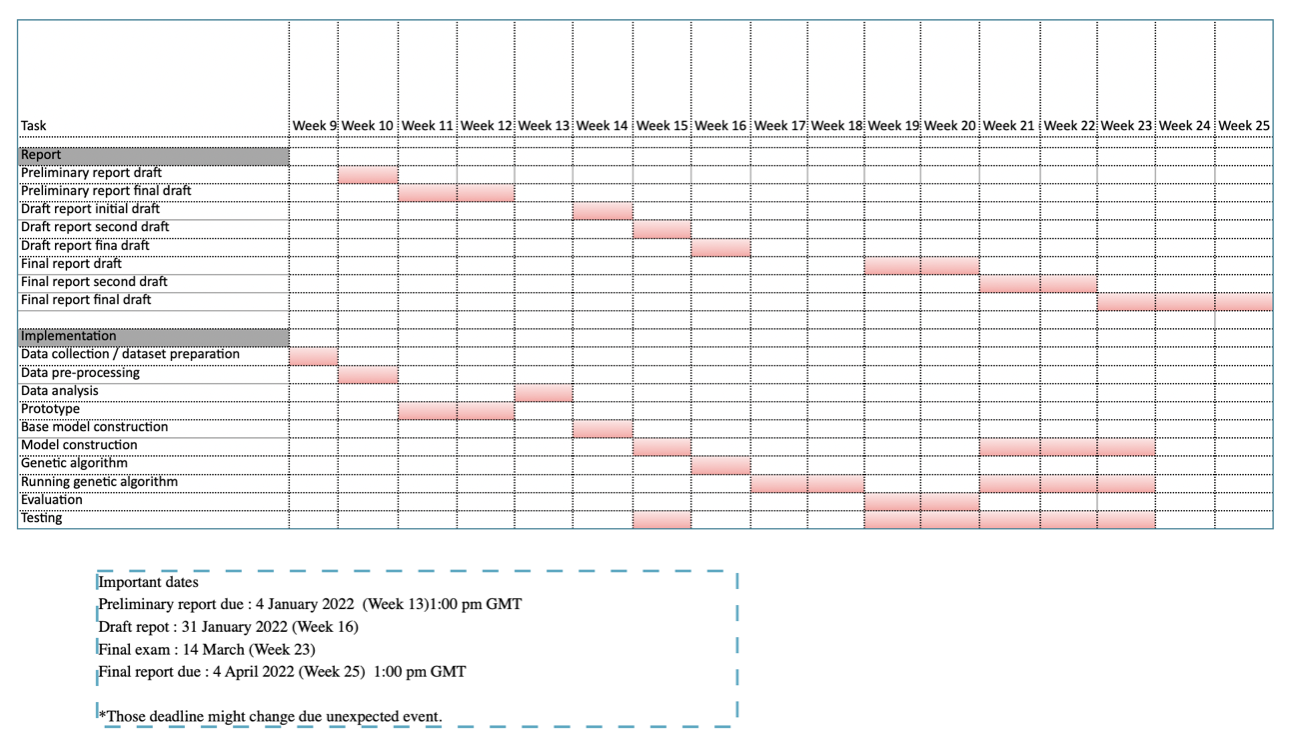
\includegraphics[width=\linewidth]{./gantt.png}
  \end{subfigure}

  \begin{subfigure}[b]{1.0\linewidth}
  \centering
  \caption{Python script to import Reddit comments}
  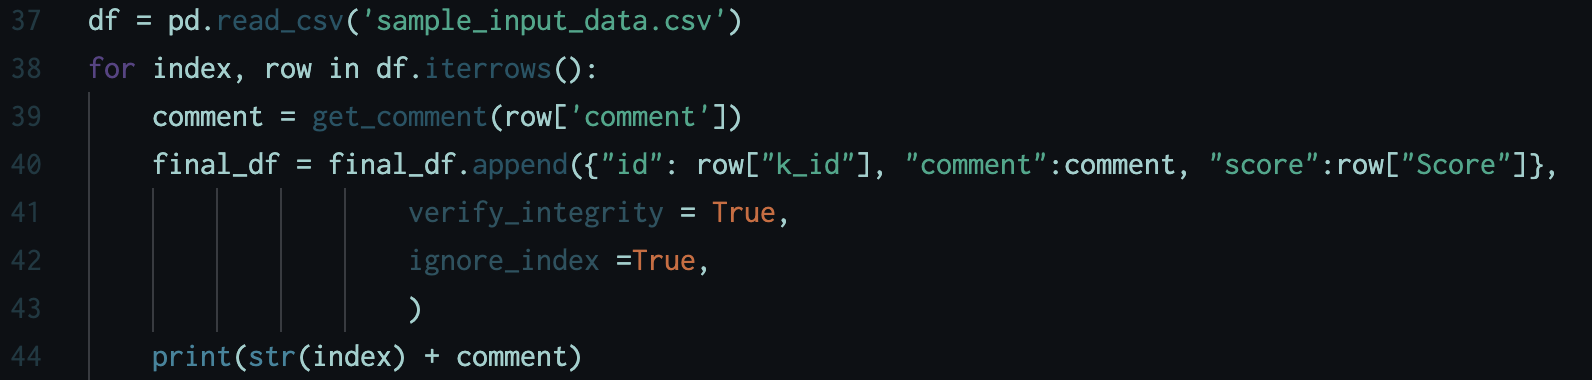
\includegraphics[width=0.5\textwidth]{./code.png}
  \end{subfigure}

  \begin{subfigure}[b]{1.0\linewidth}
  \centering
  \caption{Example of dataset}
  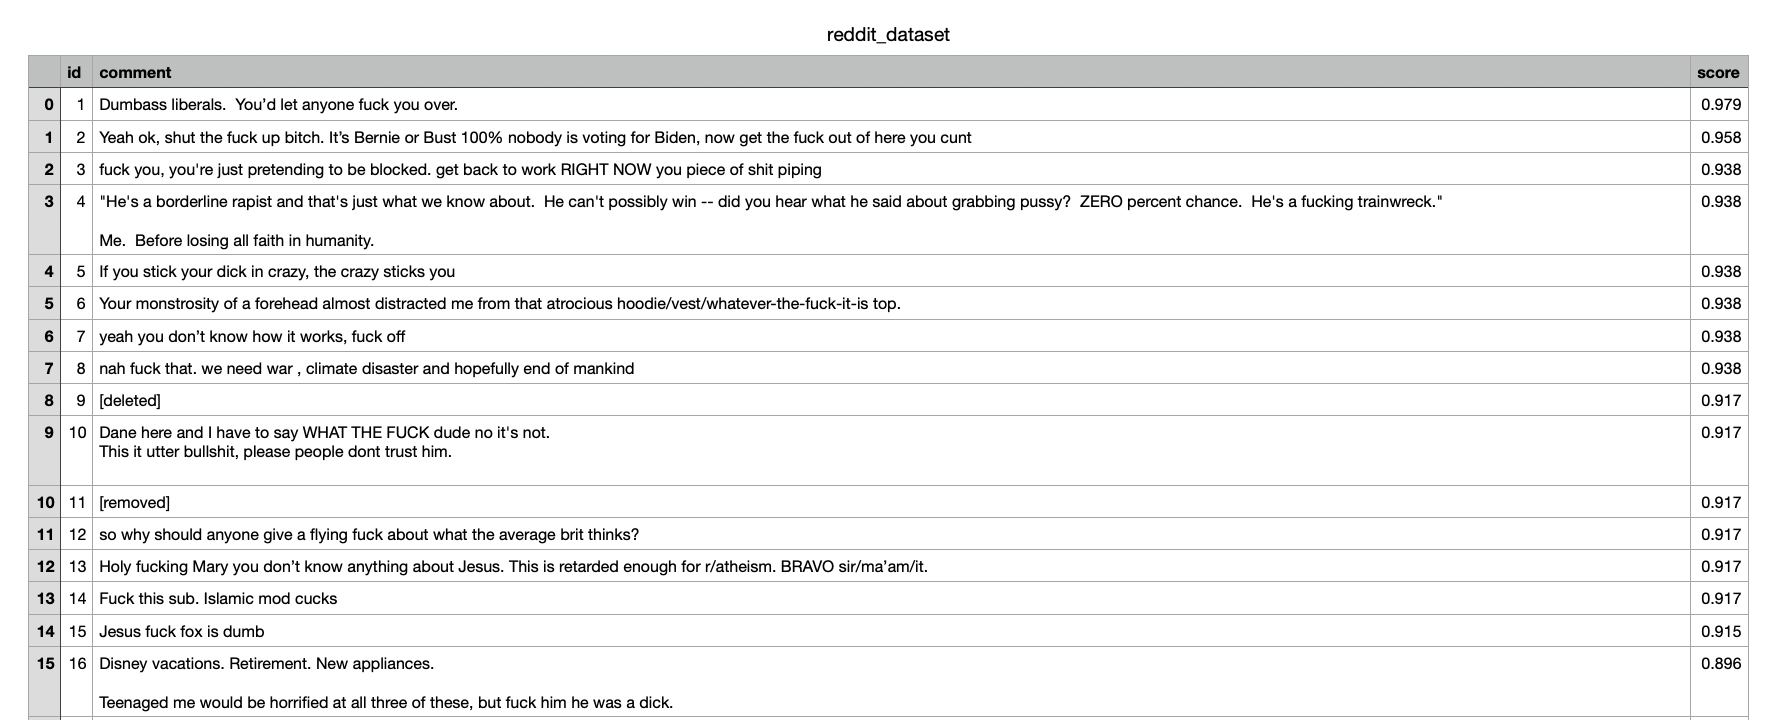
\includegraphics[width=0.5\textwidth]{./data_example.png}
  \end{subfigure}

  \begin{subfigure}[b]{1.0\linewidth}
  \centering
  \caption{Data distribution}
  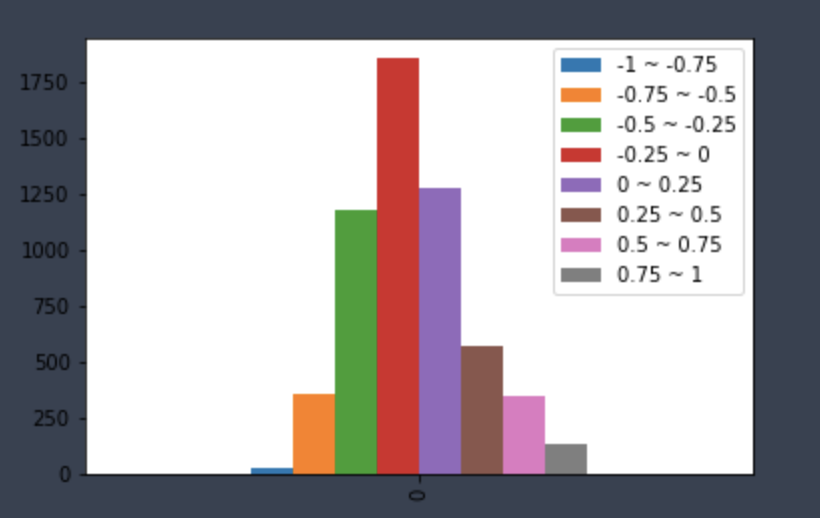
\includegraphics[width=0.5\textwidth]{./Data_distribution.png}
  \end{subfigure}
\end{figure}

\newpage

\begin{figure}[h!]\ContinuedFloat
  \centering

  \begin{subfigure}[b]{1.0\linewidth}
  \centering
  \caption{Word cloud of Reddit dataset}
  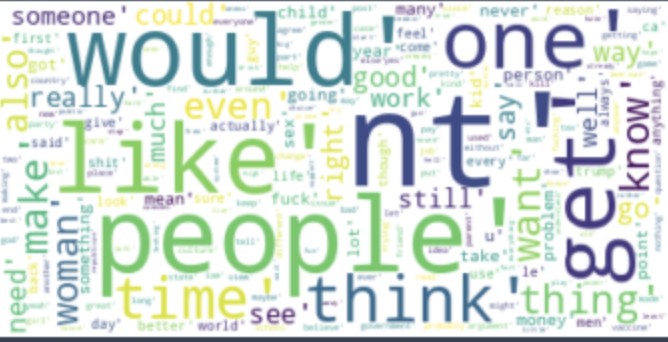
\includegraphics[width=0.5\textwidth]{./wordcloud_reddit.png}
  \end{subfigure}
  \begin{subfigure}[b]{1.0\linewidth}
  \centering
  \caption{Word cloud of offensive comments}
  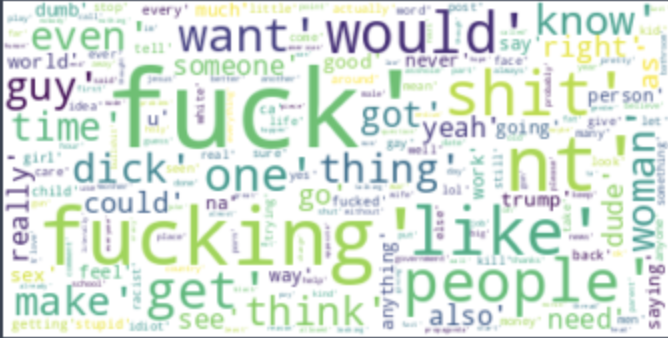
\includegraphics[width=0.5\textwidth]{./wordcloud_offensive.png}
  \end{subfigure}
  \begin{subfigure}[b]{1.0\linewidth}
  \centering
  \caption{Word cloud of }
  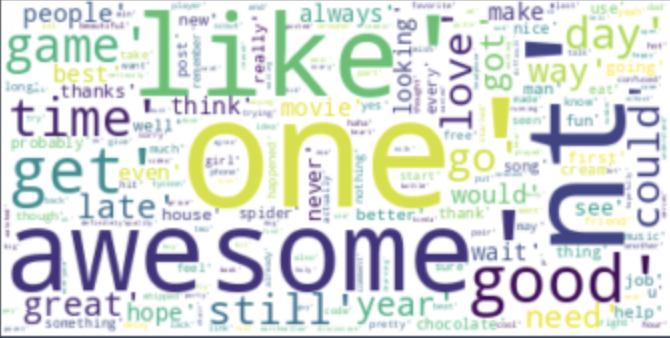
\includegraphics[width=0.5\textwidth]{./wordcloud_nonoffensive.png}
  \end{subfigure}
  \begin{subfigure}[b]{1.0\linewidth}
  \centering
  \caption{Word cloud of neutral comments}
  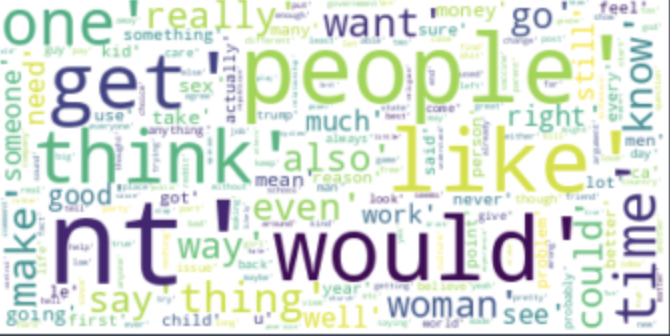
\includegraphics[width=0.5\textwidth]{./wordcloud_neutral.png}
  \end{subfigure}

\end{figure}

\newpage
\begin{figure}[h!]\ContinuedFloat
  \centering

  \begin{subfigure}[b]{1.0\linewidth}
  \centering
  \caption{Lexical diversity}
  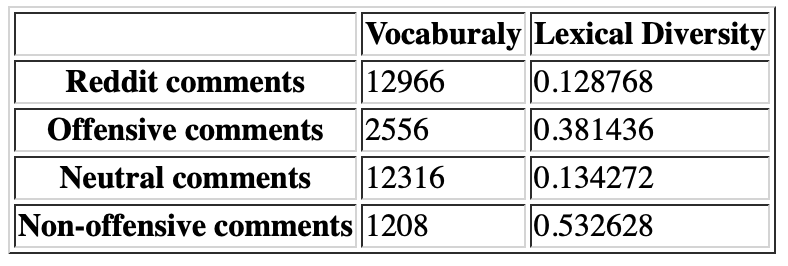
\includegraphics[width=0.5\textwidth]{./lexical_diversity.png}
  \end{subfigure}

  \begin{subfigure}[b]{1.0\linewidth}
  \centering
  \caption{Baseline model summary}
  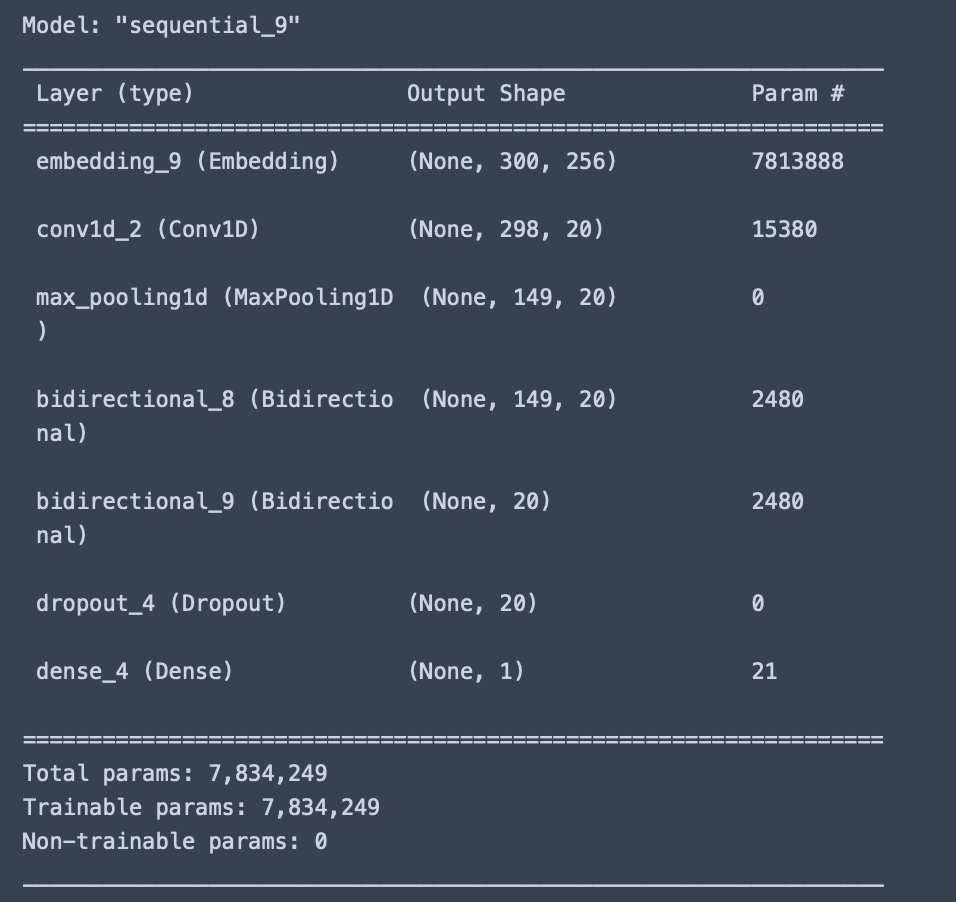
\includegraphics[width=0.5\textwidth]{./baseline_model.png}
  \end{subfigure}

  \begin{subfigure}[b]{1.0\linewidth}
  \centering
  \caption{Model 1 from GA}
  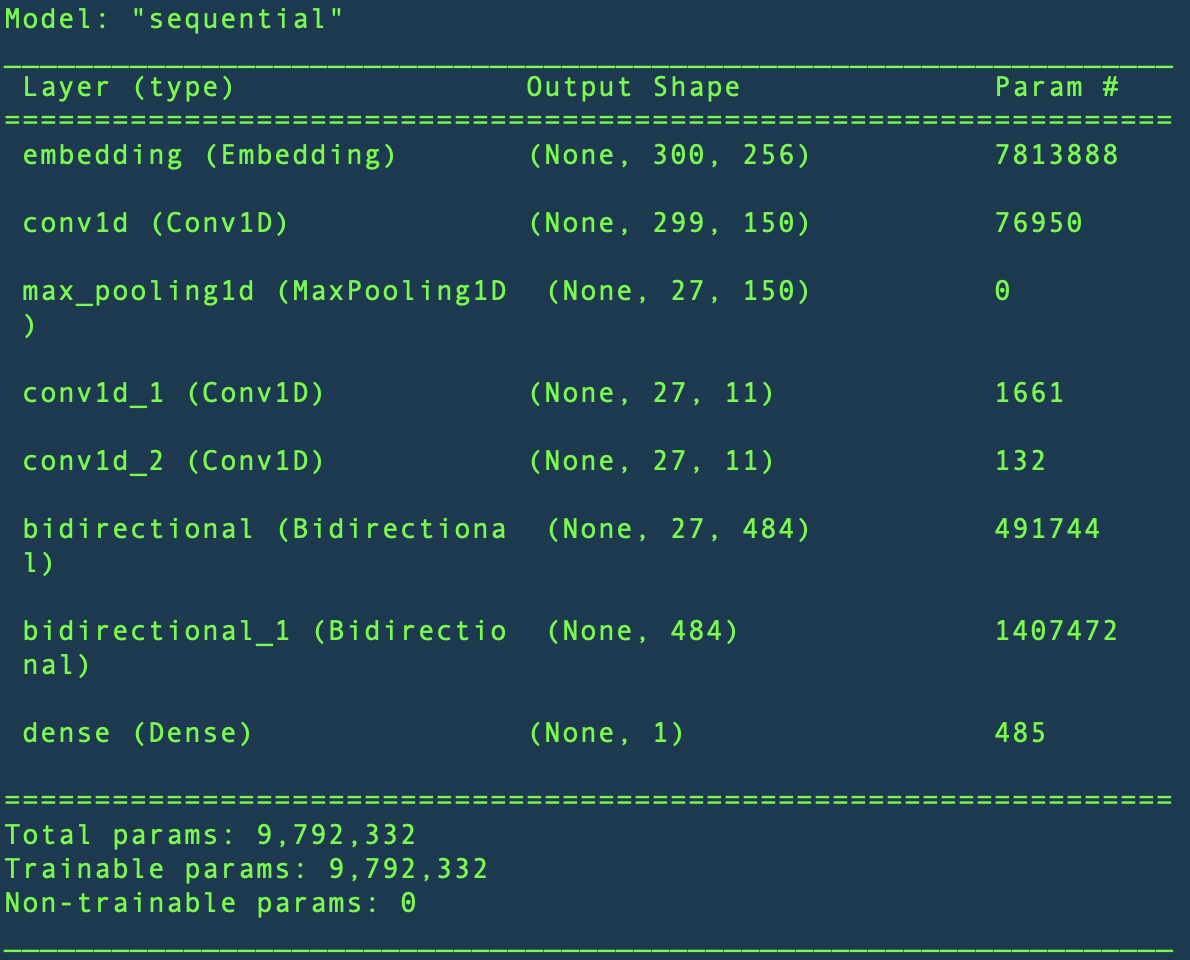
\includegraphics[width=0.5\textwidth]{./GA_model1.png}
  \end{subfigure}
\end{figure}

\newpage
\begin{figure}[h!]\ContinuedFloat
  \centering

  \begin{subfigure}[b]{1.0\linewidth}
  \centering
  \caption{Model 2 from GA}
  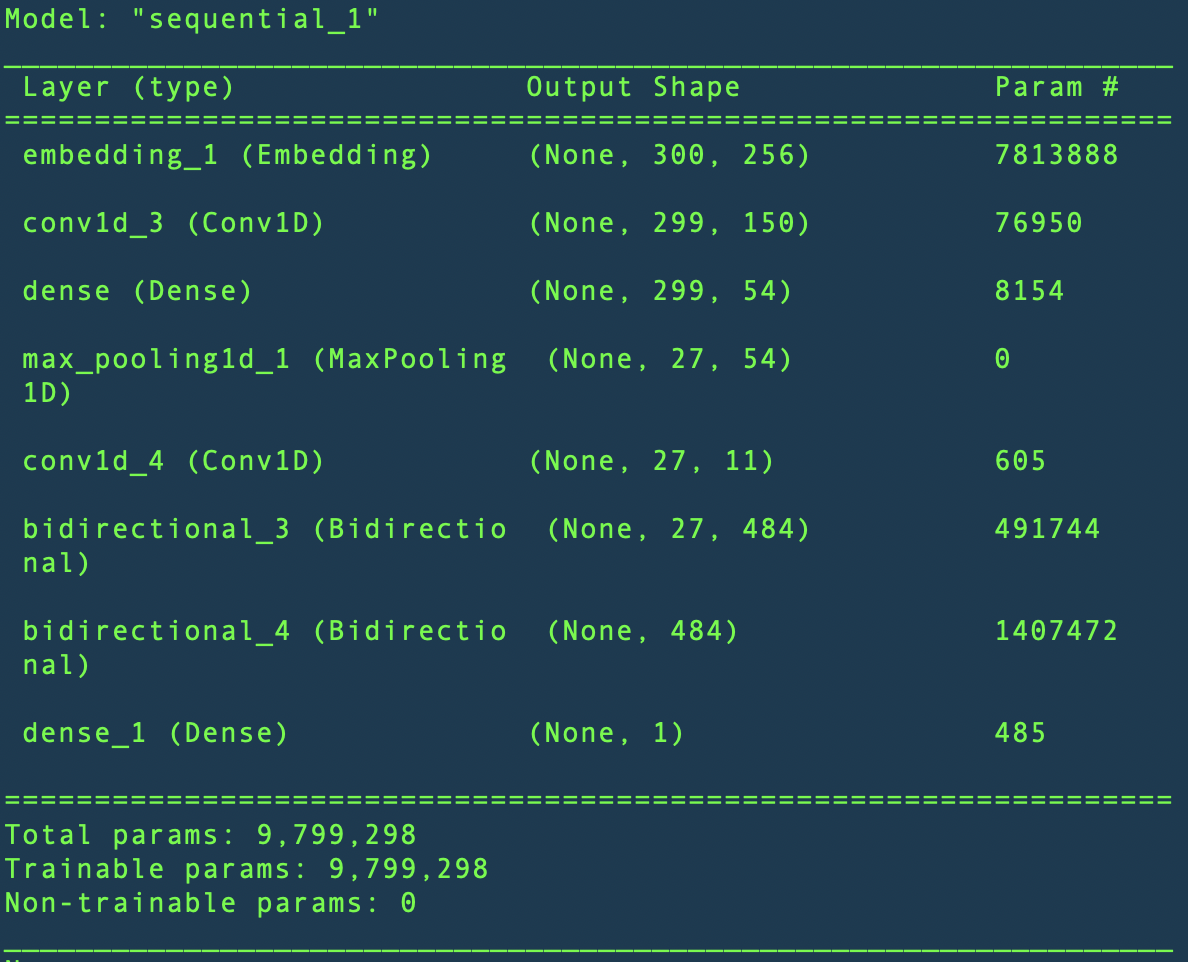
\includegraphics[width=0.5\textwidth]{./GA_model2.png}
  \end{subfigure}

  \begin{subfigure}[b]{1.0\linewidth}
  \centering
  \caption{Model 3 from GA}
  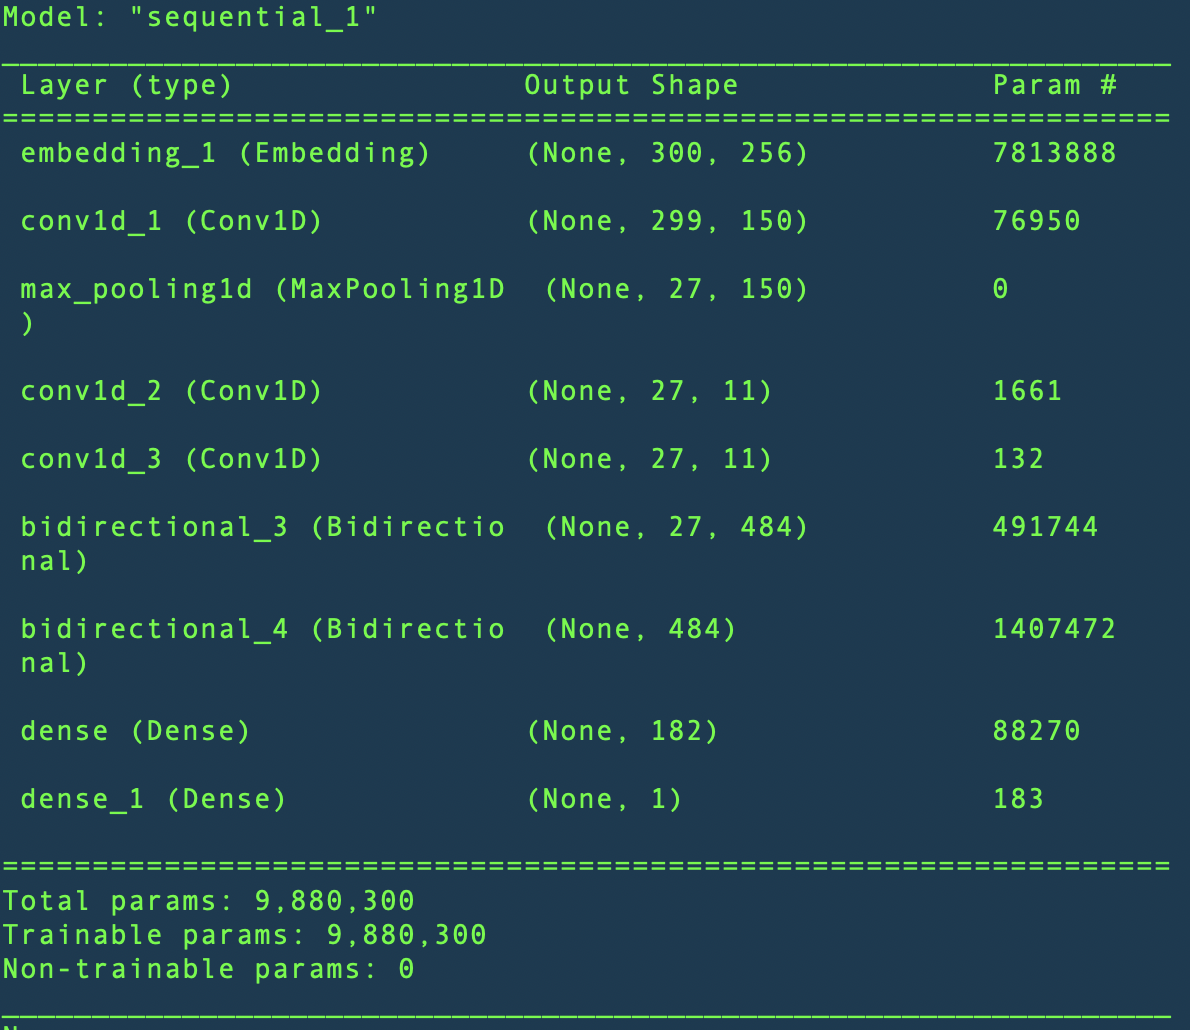
\includegraphics[width=0.5\textwidth]{./GA_model3.png}
  \end{subfigure}

  \begin{subfigure}[b]{1.0\linewidth}
  \centering
  \caption{Evaluation table}
  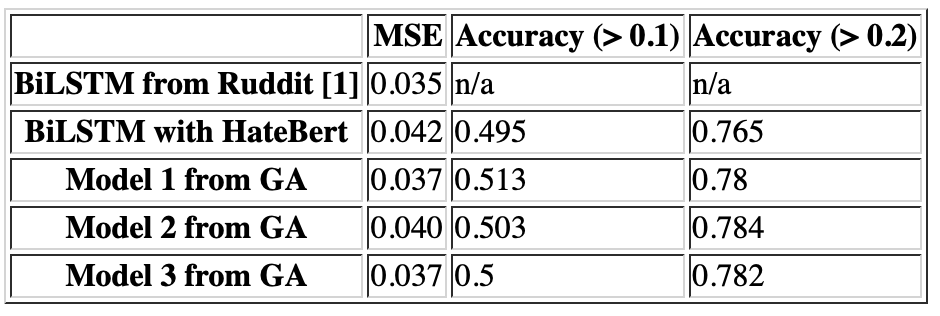
\includegraphics[width=0.5\textwidth]{./comparison_table.png}
  \end{subfigure}

\end{figure}

\newpage
\begin{figure}[h!]\ContinuedFloat
  \centering

  \begin{subfigure}[b]{1.0\linewidth}
  \centering
  \caption{Confusion Matrix of baseline model}
  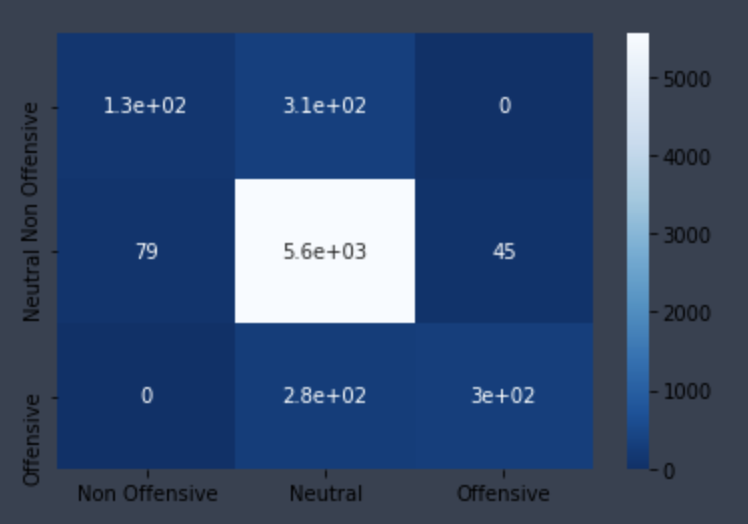
\includegraphics[width=0.5\textwidth]{./baseline_model_cm.png}
  \end{subfigure}

  \begin{subfigure}[b]{1.0\linewidth}
  \centering
  \caption{Confusion Matrix of model 1 from GA}
  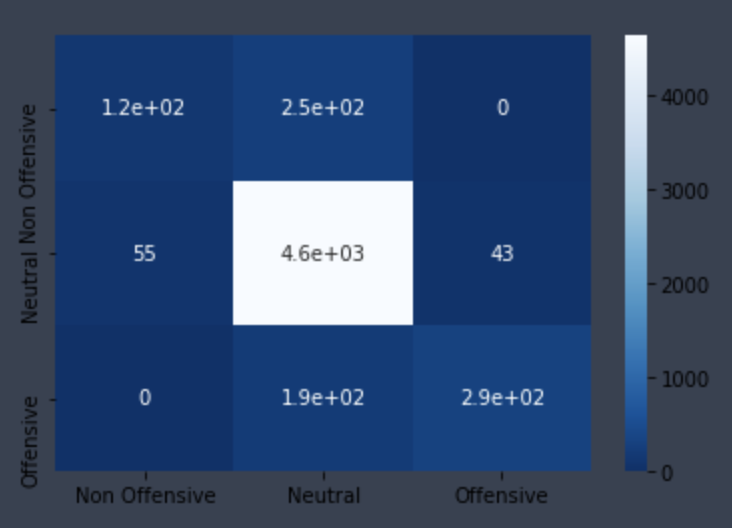
\includegraphics[width=0.5\textwidth]{./GA_model1_cm.png}
  \end{subfigure}

\end{figure}

\newpage
\begin{figure}[h!]\ContinuedFloat
  \centering

  \begin{subfigure}[b]{1.0\linewidth}
  \centering
  \caption{Confusion Matrix of model 2 from GA}
  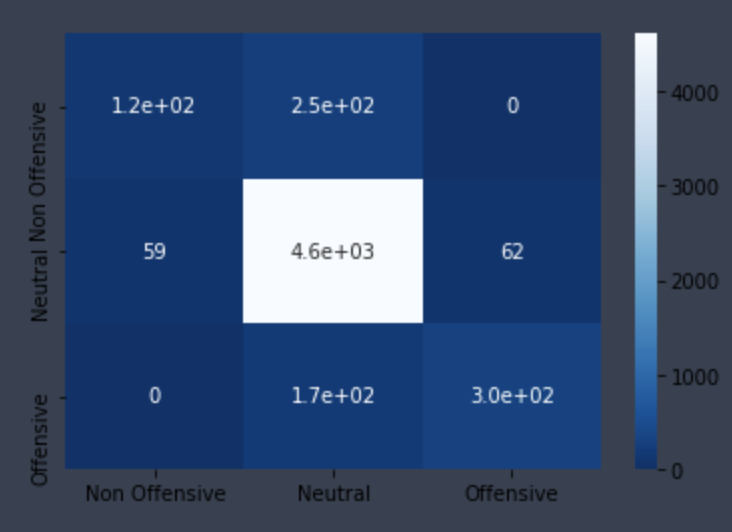
\includegraphics[width=0.5\textwidth]{./GA_model2_cm.png}
  \end{subfigure}

  \begin{subfigure}[b]{1.0\linewidth}
  \centering
  \caption{Confusion Matrix of model 3 from GA}
  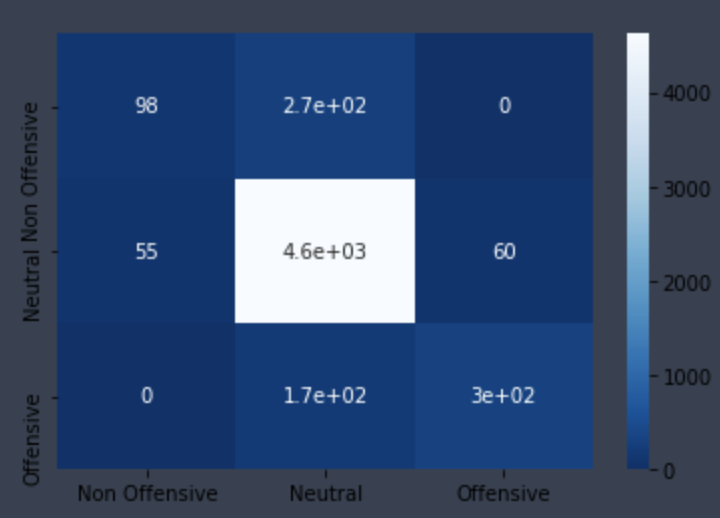
\includegraphics[width=0.5\textwidth]{./GA_model3_cm.png}
  \end{subfigure}

\end{figure}

\end{document}
